%\documentclass{standalone}
%\usepackage[utf8]{inputenc}
\usepackage[T1]{fontenc}
\usepackage[english]{babel}
%\usepackage[iso]{date}
\usepackage{microtype} % optional, for aesthetics
\usepackage{csquotes}
\usepackage{fontawesome}
%%%%%%%%%%%%%%%%%%%%%%%%%%%%%%%%%%%%
%			Bibliography			%
%%%%%%%%%%%%%%%%%%%%%%%%%%%%%%%%%%%%
\usepackage[backend=biber,style=numeric-comp,sorting=none,natbib=true]{biblatex}
\addbibresource{./BIB/Bibliography.bib}

%%%%%%%%%%%%%%%%%%%%%%%%%%%%%%%%%%%%
%			Hyperref				%
%%%%%%%%%%%%%%%%%%%%%%%%%%%%%%%%%%%%
\usepackage{hyperref}
\usepackage{lastpage}
\hypersetup{
	breaklinks=false,
	citecolor=red,
	colorlinks=true,
	linkcolor=red,
	menucolor=black,
	pdfauthor={Thomas Arne Hensel},
	urlcolor=blue,
	bookmarks=true
}
%%%%%%%%%%%%%%%%%%%%%%%%%%%%%%%%%%%%
%				math				%
%%%%%%%%%%%%%%%%%%%%%%%%%%%%%%%%%%%%
\usepackage{amsmath}
\usepackage{amssymb}
\usepackage{amsthm}
\usepackage{commath}
\usepackage{siunitx}
\usepackage{eulervm}
%
%%%%%%%%%%%%%%%%%%%%%%%%%%%%%%%%%%%%
%		Figures and Plotting		%
%%%%%%%%%%%%%%%%%%%%%%%%%%%%%%%%%%%%
%
%\graphicspath{{SECTIONS/GRAPHICS/}}
\usepackage[dvipsnames]{xcolor}
\usepackage{graphicx}
\usepackage{caption,subcaption}%for subfigures
\usepackage{standalone}%to separately produce standalone figures
\usepackage{import}%to import figures later
%
\usepackage{tikz}%drawings like geometries
\usetikzlibrary{calc,matrix,positioning}
\usetikzlibrary{decorations.pathmorphing,patterns}
\usepackage{tikzscale}
%
\usepackage{pgfplots}
\pgfplotsset{
    ,compat=newest%1.12
    }
\usepgfplotslibrary{groupplots}
\usepgflibrary{patterns}
\usepackage{pgfplotstable}
%%%%%%%%%%%%%%%%%%%%%%%%%%%%%%%%%%%%
%				Tables				%
%%%%%%%%%%%%%%%%%%%%%%%%%%%%%%%%%%%%
\usepackage{multirow}
\usepackage{lscape}
\usepackage{pdflscape}
\usepackage{rotating}
\usepackage{tabularx}
\usepackage{booktabs}
%%%%%%%%%%%%%%%%%%%%%%%%%%%%%%%%%%%%
%			print git-hash			%
%%%%%%%%%%%%%%%%%%%%%%%%%%%%%%%%%%%%
\usepackage{etoolbox}
\newtoggle{submissionBuild}
\settoggle{submissionBuild}{false}
\nottoggle{submissionBuild}{%
	\usepackage{gitver}
	\usepackage{soul}
	\sethlcolor{green}
}{}
%%%%%%%%%%%%%%%%%%%%%%%%%%%%%%%%%%%%
%			Headings				%
%%%%%%%%%%%%%%%%%%%%%%%%%%%%%%%%%%%%
\usepackage{fancyhdr}
\setlength{\headheight}{15pt}

\pagestyle{fancy}
%\renewcommand{\chaptermark}[1]{ \markboth{#1}{} }
%\renewcommand{\sectionmark}[1]{ \markright{#1} }

\fancyhf{}
\fancyhead[LE,RO]{\footnotesize{p. \thepage\ / \pageref{LastPage}}}
\fancyhead[RE]{\emph{ \nouppercase{\leftmark}} }
\fancyhead[LO]{\emph{ \nouppercase{\rightmark}} }
\fancyfoot[CE,CO]{\iftoggle{submissionBuild}{}{%
  	\noindent{\emph{Revision}\/}: \hl{\mbox{\#\gitVer}}
	}}


\fancypagestyle{plain}{ %
  \fancyhf{} % remove everything
  \renewcommand{\headrulewidth}{0pt} % remove lines as well
  \renewcommand{\footrulewidth}{0pt}
}
% This will set fancy headings to the top of the page. The page number will be
% accompanied by the total number of pages. That way, you will know if any page is missing.
% If you do not want this for your document, you can just use``\pagestyle{plain}``.
%
\usepackage{todonotes}
%----------------------
%       Own definitions and macros
%----------------------
%
%
%----------------------
%       Annotation
%----------------------
%
\newcommand{\blue}[1]{\textcolor{blue}{#1}}%for blue comments
%\DeclareUnicodeCharacter{FFFD}{\blue{XXXX}}%to find false displayed characters, e.g. in Bib
%%%%%%%%%%%%%%%%%%%%%%%%%%%%%%%%%%%%
%				math				%
%%%%%%%%%%%%%%%%%%%%%%%%%%%%%%%%%%%%
\tikzset{
declare function={
        f(\z,\v,\x) = \z+\v*\x-0.5*\g*\x^2;
        }
}
%Define IFO-Parameters
\newcommand{\tmin}{0.7}
\newcommand{\dtmax}{\dtstart}
\newcommand{\dtstart}{1.0}
\newcommand{\T}{2.0}
\newcommand{\zmin}{3.0}
\newcommand{\dvstart}{0.8}
\newcommand{\vstart}{1.0}
\newcommand{\zmax}{9.0}
\newcommand{\g}{0.6}
\newcommand{\keff}{1.0}
%
% Word like operators.
\DeclareMathOperator{\acosh}{arcosh}
\DeclareMathOperator{\arcosh}{arcosh}
\DeclareMathOperator{\arcsinh}{arsinh}
\DeclareMathOperator{\arsinh}{arsinh}
\DeclareMathOperator{\asinh}{arsinh}
\DeclareMathOperator{\card}{card}
\DeclareMathOperator{\csch}{cshs}
\DeclareMathOperator{\diam}{diam}
\DeclareMathOperator{\sech}{sech}
\renewcommand{\Im}{\mathop{{}\mathrm{Im}}\nolimits}
\renewcommand{\Re}{\mathop{{}\mathrm{Re}}\nolimits}

% Fourier transform.
\DeclareMathOperator{\fourier}{\ensuremath{\mathcal{F}}}

% Roman versions of “e” and “i” to serve as Euler's number and the imaginary
% constant.
\newcommand{\ee}{\eup}
\newcommand{\eup}{\mathrm e}
\newcommand{\ii}{\iup}
\newcommand{\iup}{\mathrm i}

% Symbols for the various mathematical fields (natural numbers, integers,
% rational numbers, real numbers, complex numbers).
\newcommand{\C}{\ensuremath{\mathbb C}}
\newcommand{\N}{\ensuremath{\mathbb N}}
\newcommand{\Q}{\ensuremath{\mathbb Q}}
\newcommand{\R}{\ensuremath{\mathbb R}}
\newcommand{\Z}{\ensuremath{\mathbb Z}}

% Shape like operators.
\DeclareMathOperator{\dalambert}{\Box}
\DeclareMathOperator{\laplace}{\bigtriangleup}
\newcommand{\curl}{\vnabla \times}
\newcommand{\divergence}[1]{\inner{\vnabla}{#1}}
\newcommand{\vnabla}{\vec \nabla}

\newcommand{\half}{\frac 12}

% Unit vector (German „Einheitsvektor“).
\newcommand{\ev}{\hat{\vec e}}

% Scientific notation for large numbers.
\newcommand{\e}[1]{\cdot 10^{#1}}

% Mathematician's notation for the inner (scalar, dot) product.
\newcommand{\inner}[2]{\left\langle #1, #2 \right\rangle}

% Placeholders.
\newcommand{\emesswert}{\del{\messwert \pm \messwert}}
\newcommand{\fehlt}{\textcolor{darkred}{Hier fehlen noch Inhalte.}}
\newcommand{\messwert}{\textcolor{blue}{\square}}
\newcommand{\punkte}{\textcolor{white}{xxxxx}}

% Separator for equations on a single line.
\newcommand{\eqnsep}{,\quad}

% Quantum Mechanics
\newcommand{\bra}[1]{\left\langle #1 \right|}
\newcommand{\ket}[1]{\left| #1 \right\rangle}
\newcommand{\braket}[2]{\left\langle #1 \left. \vphantom{#1 #2} \right| #2 \right\rangle}
%\begin{document}

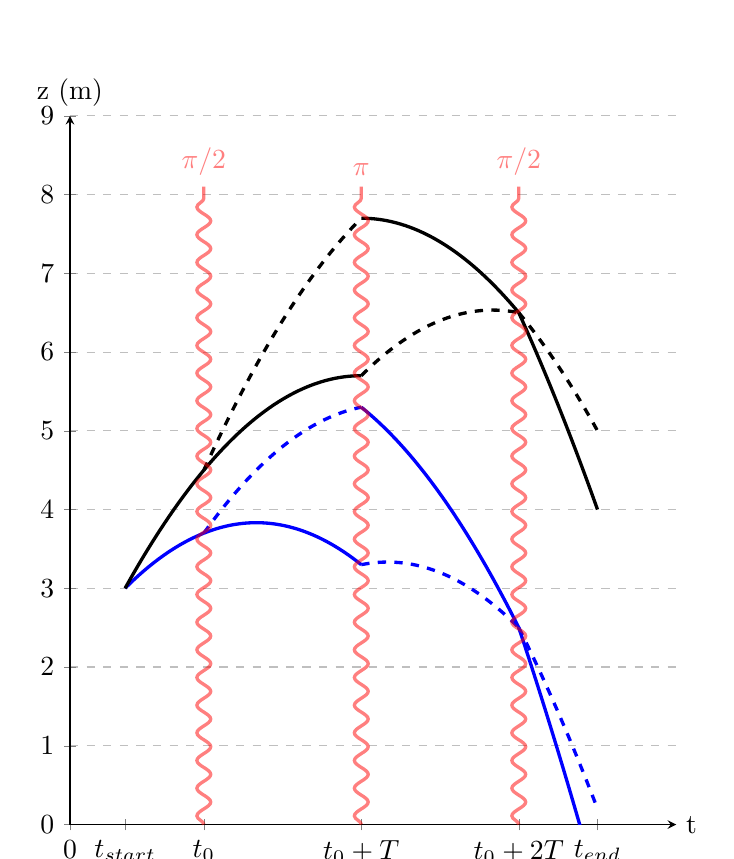
\begin{tikzpicture}
%
\begin{axis}[
    %title={Dual-species Mach-Zehnder atom interferometer},
    xlabel={t}, xlabel style={at={(1,0)}, anchor=west},
    ylabel={z (m)}, ylabel style={rotate=-90,at={(0,1)}, anchor=south},
    xmin=0.0, xmax=\tmin+\dtstart+2*\T+2*\dtmax,
    ymin=0, ymax=\zmax,
    axis lines = left,
    y=1.cm,
    x=1.cm,
    xtick={0,0.7,1.7,3.7,5.7,6.7},%{0,\tmin,\tmin+\dtstart,\tmin+\dtstart+\T,\tmin+\dtstart+\T+\T,\tmin+\dtstart+\T+\T+\dtmax},
    xticklabels={$0$,$t_{start}$,$t_0$,$t_0+T$,$t_0+2T$,$t_{end}$},
    ytick={0,1,...,12},
    legend pos=north west,
    %grid=both,
    ymajorgrids=true,
    grid style=dashed,
    ]
    %upper path
    \addplot[color=blue, samples=50, very thick][domain=\tmin:\tmin+\dtstart]{
        f(
        \zmin
        ,\vstart
        ,(x-\tmin)
        )
    };
    \addplot[color=blue, samples=50, very thick, dashed][domain=\tmin+\dtstart:\tmin+\dtstart+\T]{
        f(
            f(\zmin,\vstart,\dtstart)
            ,\vstart-\g*\dtstart+\keff
            ,x-\tmin-\dtstart
        )
    };
    \addplot[color=blue, samples=50, very thick][domain=\tmin+\dtstart+\T:\tmin+\dtstart+\T+\T]{
        f(
            f(f(\zmin,\vstart,\dtstart),\vstart-\g*\dtstart+\keff,\T)
            ,\vstart-\g*(\dtstart+\T)
            ,x-\tmin-\dtstart-\T
            )
    };
    %lower path
    \addplot[color=blue, samples=50, very thick][domain=\tmin+\dtstart:\tmin+\dtstart+\T]{
        f(
            f(\zmin,\vstart,\dtstart)
            ,\vstart-\g*\dtstart
            ,x-\tmin-\dtstart
        )
    };
    \addplot[color=blue, samples=50, very thick, dashed][domain=\tmin+\dtstart+\T:\tmin+\dtstart+\T+\T]{
        f(
            f(f(\zmin,\vstart,\dtstart),\vstart-\g*\dtstart,\T)
            ,\vstart-\g*(\dtstart+\T)+\keff
            ,x-\tmin-\dtstart-\T
        )
    };
    \addplot[color=blue, samples=50, very thick, dashed][domain=\tmin+\dtstart+2*\T:\tmin+\dtstart+\T+\T+\dtmax]{
        f(
            f(f(f(\zmin,\vstart,\dtstart),\vstart-\g*\dtstart,\T),\vstart-\g*(\dtstart+\T)+\keff,\T)
            ,\vstart-\g*(\dtstart+\T+\T)
            ,x-\tmin-\dtstart-\T-\T
        )
    };
    \addplot[color=blue, samples=50, very thick][domain=\tmin+\dtstart+2*\T:\tmin+\dtstart+\T+\T+\dtmax]{
        f(
            f(f(f(\zmin,\vstart,\dtstart),\vstart-\g*\dtstart,\T),\vstart-\g*(\dtstart+\T)+\keff,\T)
            ,\vstart-\g*(\dtstart+\T+\T)-\keff
            ,x-\tmin-\dtstart-\T-\T
        )
    };    
    %upper path
    \addplot[color=black, samples=50, very thick][domain=\tmin:\tmin+\dtstart]{
        f(
        \zmin
        ,\vstart+\dvstart
        ,(x-\tmin)
        )
    };
    \addplot[color=black, samples=50, very thick, dashed][domain=\tmin+\dtstart:\tmin+\dtstart+\T]{
        f(
            f(\zmin,\vstart+\dvstart,\dtstart)
            ,\vstart+\dvstart-\g*\dtstart+\keff
            ,x-\tmin-\dtstart
        )
    };
    \addplot[color=black, samples=50, very thick][domain=\tmin+\dtstart+\T:\tmin+\dtstart+\T+\T]{
        f(
            f(f(\zmin,\vstart+\dvstart,\dtstart),\vstart+\dvstart-\g*\dtstart+\keff,\T)
            ,\vstart+\dvstart-\g*(\dtstart+\T)
            ,x-\tmin-\dtstart-\T
            )
    };
    %lower path
    \addplot[color=black, samples=50, very thick][domain=\tmin+\dtstart:\tmin+\dtstart+\T]{
        f(
            f(\zmin,\vstart+\dvstart,\dtstart)
            ,\vstart+\dvstart-\g*\dtstart
            ,x-\tmin-\dtstart
        )
    };
    \addplot[color=black, samples=50, very thick, dashed][domain=\tmin+\dtstart+\T:\tmin+\dtstart+\T+\T]{
        f(
            f(f(\zmin,\vstart+\dvstart,\dtstart),\vstart+\dvstart-\g*\dtstart,\T)
            ,\vstart+\dvstart-\g*(\dtstart+\T)+\keff
            ,x-\tmin-\dtstart-\T
        )
    };
    \addplot[color=black, samples=50, very thick][domain=\tmin+\dtstart+2*\T:\tmin+\dtstart+\T+\T+\dtmax]{
        f(
            f(f(f(\zmin,\vstart+\dvstart,\dtstart),\vstart+\dvstart-\g*\dtstart,\T),\vstart+\dvstart-\g*(\dtstart+\T)+\keff,\T)
            ,\vstart+\dvstart-\g*(\dtstart+\T+\T)-\keff
            ,x-\tmin-\dtstart-\T-\T
        )
    };  
    \addplot[color=black, samples=50, very thick, dashed][domain=\tmin+\dtstart+2*\T:\tmin+\dtstart+\T+\T+\dtmax]{
        f(
            f(f(f(\zmin,\vstart+\dvstart,\dtstart),\vstart+\dvstart-\g*\dtstart,\T),\vstart+\dvstart-\g*(\dtstart+\T)+\keff,\T)
            ,\vstart+\dvstart-\g*(\dtstart+\T+\T)
            ,x-\tmin-\dtstart-\T-\T
        )
    };  
\end{axis}

    %create Laserbeams
    \draw[decorate, decoration = snake, very thick, red, opacity=0.5]
    ({\tmin + \dtstart},0) to ({\tmin + \dtstart},{.9*\zmax}) node[above] {$\pi/2$};
    \draw[decorate, decoration = snake, very thick, red, opacity=0.5,] 
    ({\tmin + \dtstart+\T},0) to ({\tmin + \dtstart + \T},{.9*\zmax}) node[above] {$\pi$};
    \draw[decorate, decoration = snake, very thick, red, opacity=0.5,] 
    ({\tmin + \dtstart + 2*\T},0) to ({\tmin + \dtstart + 2*\T},{.9*\zmax}) node[above] {$\pi/2$};
\end{tikzpicture}
%\end{document}